% ============================================================
%  Part II — System architecture diagram (standalone)
%  Ambulance detector (C++ HOG+SVM) <-> Telegram bot (Python YOLO-seg)
%  Compile:  pdflatex arquitectura.tex
%  Rasterize: pdftoppm -png -r 200 arquitectura.pdf arquitectura
% ============================================================
\documentclass[border=10pt]{standalone}
\usepackage[utf8]{inputenc}
\usepackage[T1]{fontenc}
\usepackage{lmodern}
\usepackage{tikz}
\usetikzlibrary{shapes.geometric, arrows.meta, positioning, fit,
                backgrounds, calc}

\definecolor{salesiana}{RGB}{0, 84, 166}
\definecolor{accentgreen}{RGB}{34, 139, 34}
\definecolor{accentorange}{RGB}{204, 85, 0}

\begin{document}
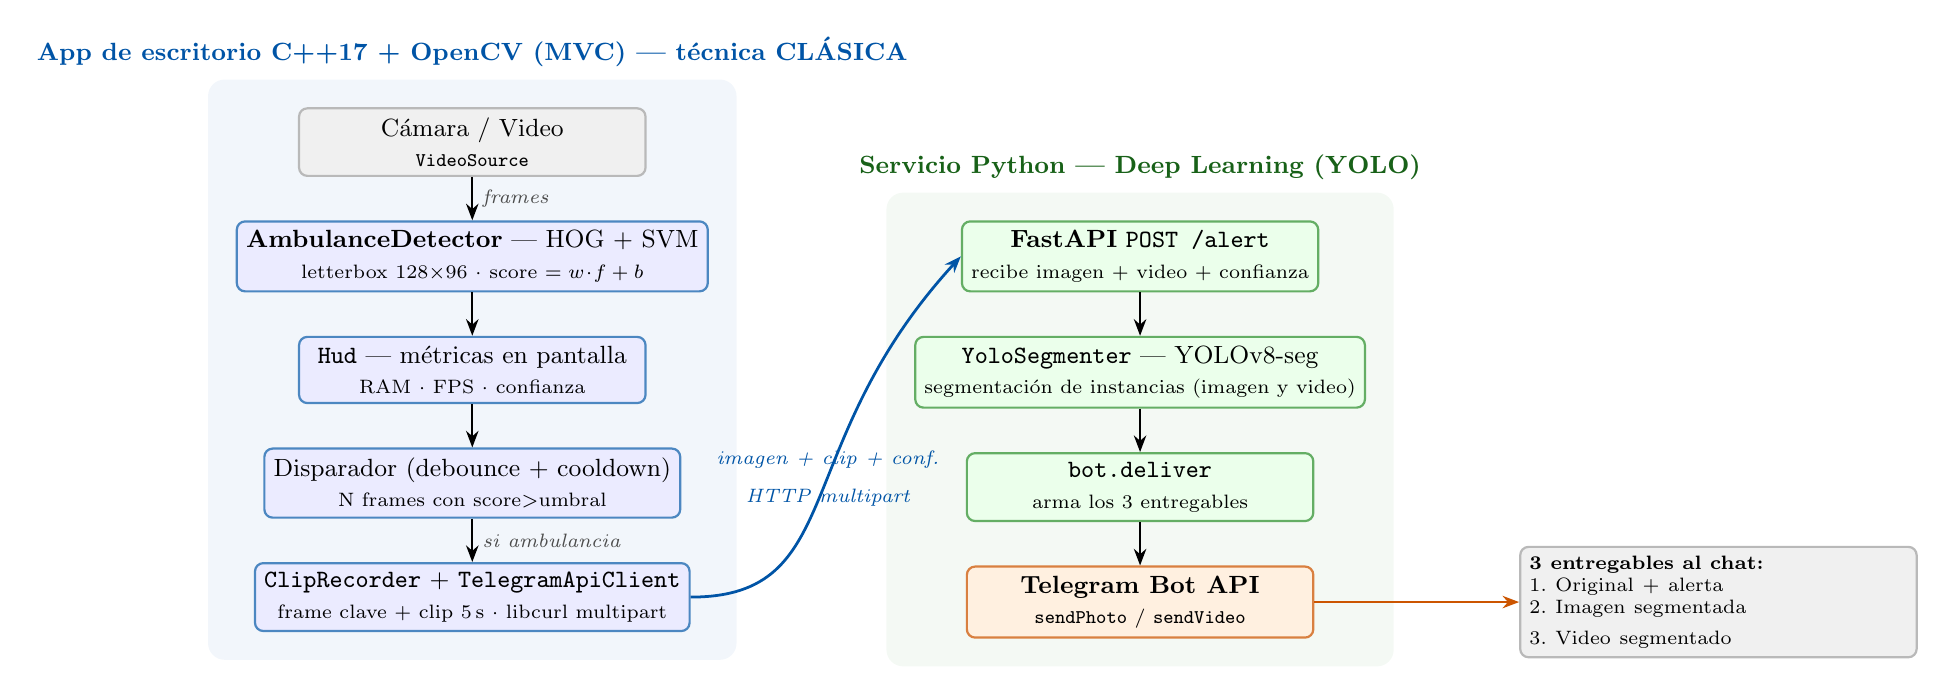
\begin{tikzpicture}[
    node distance = 0.55cm,
    box/.style   = {rectangle, rounded corners=3pt, minimum width=4.4cm,
                    minimum height=0.82cm, align=center, font=\small,
                    draw, thick},
    cpp/.style   = {box, fill=blue!8,   draw=salesiana!70},
    py/.style    = {box, fill=green!8,  draw=accentgreen!70},
    io/.style    = {box, fill=gray!12,  draw=gray!55},
    tg/.style    = {box, fill=orange!12, draw=accentorange!75},
    arr/.style   = {-{Stealth[length=6pt]}, thick},
    lbl/.style   = {font=\scriptsize\itshape, text=gray!60!black},
    grp/.style   = {rounded corners=6pt, inner sep=10pt}
]

% ---- C++ column (classical detector) ----
\node[io]  (src)  {Cámara / Video \\ {\scriptsize \texttt{VideoSource}}};
\node[cpp, below=of src] (det) {\textbf{AmbulanceDetector} — HOG + SVM \\
      {\scriptsize letterbox 128$\times$96 $\cdot$ score $=w\!\cdot\!f+b$}};
\node[cpp, below=of det] (hud) {\texttt{Hud} — métricas en pantalla \\
      {\scriptsize RAM $\cdot$ FPS $\cdot$ confianza}};
\node[cpp, below=of hud] (trig){Disparador (debounce + cooldown) \\
      {\scriptsize N frames con score$>$umbral}};
\node[cpp, below=of trig] (rec) {\texttt{ClipRecorder} + \texttt{TelegramApiClient} \\
      {\scriptsize frame clave + clip 5\,s $\cdot$ libcurl multipart}};

% ---- Python column (deep-learning segmentation) ----
\node[py, right=3.2cm of det] (api) {\textbf{FastAPI} \texttt{POST /alert} \\
      {\scriptsize recibe imagen + video + confianza}};
\node[py, below=of api] (yolo) {\texttt{YoloSegmenter} — YOLOv8-seg \\
      {\scriptsize segmentación de instancias (imagen y video)}};
\node[py, below=of yolo] (deliver) {\texttt{bot.deliver} \\
      {\scriptsize arma los 3 entregables}};
\node[tg, below=of deliver] (tgram) {\textbf{Telegram Bot API} \\
      {\scriptsize \texttt{sendPhoto} / \texttt{sendVideo}}};

% ---- vertical flows ----
\draw[arr] (src)  -- node[lbl,right]{frames} (det);
\draw[arr] (det)  -- (hud);
\draw[arr] (hud)  -- (trig);
\draw[arr] (trig) -- node[lbl,right]{si ambulancia} (rec);
\draw[arr] (api)   -- (yolo);
\draw[arr] (yolo)  -- (deliver);
\draw[arr] (deliver) -- (tgram);

% ---- HTTP boundary (C++ -> Python) ----
\draw[arr, salesiana, line width=1pt]
  (rec.east) .. controls +(2.0,0) and +(-2.2,-2.4) ..
  node[lbl, below, pos=0.55, text=salesiana]{HTTP multipart}
  node[lbl, above, pos=0.55, text=salesiana]{imagen + clip + conf.}
  (api.west);

% ---- Telegram deliverables ----
\node[io, right=2.6cm of tgram, text width=4.8cm, align=left]
  (out) {\scriptsize \textbf{3 entregables al chat:}\\ 1.~Original + alerta\\ 2.~Imagen segmentada\\ 3.~Video segmentado};
\draw[arr, accentorange] (tgram.east) -- (out.west);

% ---- group frames ----
\begin{scope}[on background layer]
  \node[grp, fill=salesiana!5, fit=(src)(det)(hud)(trig)(rec)] (cbox) {};
  \node[grp, fill=accentgreen!5, fit=(api)(yolo)(deliver)(tgram)] (pbox) {};
\end{scope}
\node[font=\small\bfseries, text=salesiana, above=1pt of cbox.north] {App de escritorio C++17 + OpenCV (MVC) — técnica CLÁSICA};
\node[font=\small\bfseries, text=accentgreen!70!black, above=1pt of pbox.north] {Servicio Python — Deep Learning (YOLO)};

\end{tikzpicture}
\end{document}
